\chapter{Exploratory: what the law permits for gravitational engineering}\label{ch:exploratory}

\section*{The place}
This chapter is written for fun. It shows how wide the reach of IAM's Law is, from the cosmic horizon down to a spacecraft, and
nothing in it is offered as a validated result or a proposal to build anything. It is an exploratory chapter, not a validation chapter. It is divided into two explicitly separated zones. Zone~I contains only results that follow
rigorously from established physics (general relativity, the equivalence principle, expansion kinematics) combined with the already-stated
identifications of IAM. Every equation in Zone~I is derivable and is either standard physics or follows from the structure of IAM stated in
Part~\ref{part:2}. Zone~II is conjectural. It begins at an explicitly marked transition and concerns a regime that requires a material whose existence
is not established. No equation in Zone~II is claimed as derived; each is presented as the form a future derivation would have to take, conditional on
premises that are stated as premises. The boundary between what is established and what is conjectured is never blurred. This separation is the
entire point of the chapter. Nothing in this chapter is used anywhere else in the book.

\section{Premise: what IAM already says about gravity}\label{sec:ge_premise}
IAM leaves general relativity as it is. At each irreversible quantum-to-classical transition (decoherence) on a timelike worldline, classical
information is produced and paid for at the Landauer cost~\cite{Landauer1961}
\begin{equation}
\Delta E_{\rm rec}=\kB T_H\ln2\ \text{per bit},\qquad T_H=\frac{\hbar H}{2\pi\kB},
\label{eq:ge_landauer}
\end{equation}
where $T_H$ is the (Gibbons--Hawking) horizon temperature~\cite{GibbonsHawking1977} (Chapter~\ref{ch:theory}). Today $T_H=2.65\times10^{-30}$\,K and
$\kB T_H\ln2=2.53\times10^{-53}$\,J per bit at the photon-sector $H_0=67.16$\,km\,s$^{-1}$\,Mpc$^{-1}$, and $2.85\times10^{-30}$\,K and
$2.72\times10^{-53}$\,J at the matter-sector $H_0=72.26$. \calc

This cost is partitioned by the virial theorem into two equal halves (Chapter~\ref{ch:virial_law}): a geometric/potential half that manifests locally
as the gravitational potential, and a kinetic/informational half that manifests globally as the dark-energy term in the expansion
(Chapter~\ref{ch:virial_partners}). \interp{} The partition is fixed at $1/2$ by the equilibrium condition (the coupling constant
$\beta_m=\Omega_m/2=0.15765$, Chapter~\ref{ch:virial}), \derived{} and the cumulative record is encoded in the activation function
\begin{equation}
E(a)=\exp\!\left(1-\frac1a\right),\qquad E(1)=1,\qquad E(a\to\infty)=e,
\label{eq:ge_Ea}
\end{equation}
whose rate $\mathrm dE/\mathrm d\ln a=E/a$ peaks at $a=1$, \derived{} entering the matter-sector expansion as
\begin{equation}
H^2_{\rm eff,m}(a)=H^2_{\Lambda{\rm CDM}}(a)+\beta_m\,E(a)\,H_0^2 .
\label{eq:ge_Hm}
\end{equation}
These are not new to this chapter; they are the established core of IAM and are tested against data in Part~\ref{part:2}. The present chapter asks a
single question: taking these as given, what does the framework permit?

\section{Zone I: established physics and IAM consequences}\label{sec:ge_zone1}

\subsection{Gravity as a steerable effective potential}
In IAM the locally felt gravitational acceleration is the gradient of an effective potential built from the potential half of the partition:
\begin{equation}
\mathbf g_{\rm IAM}(\mathbf x)=-\nabla\Phi_{\rm IAM}(\mathbf x).
\label{eq:ge_g}
\end{equation}
This is definitional and recovers Newtonian gravity in the weak field. \derived{} The content of Zone~I is the following: whatever physical process
sets $\Phi_{\rm IAM}$, a body responds only to its local gradient. Equation~\eqref{eq:ge_g} is the only ingredient required for the kinematic results
below. How $\Phi_{\rm IAM}$ might be engineered is not asked yet; that is Zone~II. The question here is only what follows if the gradient can be shaped.
Whether it can is the question of Zone~II.

\subsection{Free-fall motion carries no felt acceleration (equivalence principle)}\label{sec:ge_freefall}
A body moving solely under $\mathbf g_{\rm IAM}$ follows a geodesic. Its equation of motion is
\begin{equation}
\ddot{\mathbf x}=-\nabla\Phi_{\rm IAM}(\mathbf x).
\label{eq:ge_eom}
\end{equation}
Every part of the body, and any occupant, obeys the same equation. By the equivalence principle (established physics since 1907), an observer in free
fall experiences no proper acceleration: the locally felt force is
\begin{equation}
\mathbf f_{\rm felt}=m\left(\ddot{\mathbf x}+\nabla\Phi_{\rm IAM}\right)=0,
\label{eq:ge_felt}
\end{equation}
identically, regardless of the magnitude or direction of $\nabla\Phi_{\rm IAM}$, provided the gradient is uniform across the body's scale $L$.
\derived{} The residual tidal force is the differential of the gradient,
\begin{equation}
f_{\rm tidal}\sim mL\,\partial^2\Phi_{\rm IAM},
\label{eq:ge_tidal}
\end{equation}
and vanishes in the limit of a gradient uniform over $L$. For a point mass $M$ at distance $r$, $\Phi=-GM/r$ and $g(r)-g(r+L)=2GML/r^3$ to first
order in $L$, which is $L\,|\partial_r^2\Phi|$. \derived{} At the Earth's surface this is $3.1\times10^{-6}\,g$ across 10\,m and
$3.1\times10^{-5}\,g$ across 100\,m (Figure~\ref{fig:transit}b). \calc

\emph{Consequence (rigorous).} A craft that moves by following a shaped $\Phi_{\rm IAM}$ gradient undergoes no felt acceleration during arbitrary
changes of speed or direction. A $90^\circ$ ``turn'' is accomplished by relocating the gradient direction; the craft and occupants remain in free fall
throughout and feel nothing beyond the tidal term. This dissolves the inertial objection to abrupt high-acceleration maneuvers. It is a direct
consequence of the equivalence principle and requires no new physics. \derived{} (conditional on a shaped gradient) How a gradient could be moved is the question of Zone~II.

\subsection{The hover and the abrupt departure as gradient operations}
Write the potential as an ambient part and an engineered part, $\Phi=\Phi_{\rm amb}+\Phi_{\rm IAM}$, with $\mathbf g_{\rm amb}=-\nabla\Phi_{\rm amb}$.
A stationary hover corresponds to shaping $\Phi_{\rm IAM}$ so that its gradient cancels the ambient gravitational gradient,
\begin{equation}
\nabla\Phi_{\rm IAM}=\mathbf g_{\rm amb}=-\nabla\Phi_{\rm amb},\qquad -\nabla\left(\Phi_{\rm amb}+\Phi_{\rm IAM}\right)=0 ,
\label{eq:ge_hover}
\end{equation}
leaving the craft in a local null. \derived{} An abrupt departure corresponds to a steep gradient placed along the departure direction; the craft
free-falls into it with coordinate acceleration $|\nabla\Phi_{\rm IAM}|$ but, by Section~\ref{sec:ge_freefall}, zero felt acceleration. Both are the
same operation (shaping the gradient) at different settings. No equation here exceeds Newtonian gravity plus the equivalence principle. \derived{}
(conditional on a shaped gradient)

\subsection{Orientation along the gradient}\label{sec:ge_orient}
A rigid body suspended in a gradient orients so that its constrained axis aligns with the local ``down'' defined by $-\nabla\Phi_{\rm IAM}$, exactly as
a plumb bob hangs toward the net field. Its hang angle from the vertical is
\begin{equation}
\theta=\arctan\!\left(\frac{|\nabla\Phi_{\rm IAM}|_{\rm horizontal}}{|\nabla\Phi_{\rm IAM}|_{\rm vertical}}\right),
\label{eq:ge_plumb}
\end{equation}
the same as a plumb line in a frame with horizontal acceleration $a_h$ and vertical field $g_v$, $\tan\theta=a_h/g_v$ ($5.7^\circ$ at $a_h=0.1\,g$).
\derived{} (suspended body) The angle exists because the suspension pulls on the body.

A craft in free fall is not suspended. In a uniform gradient every mass element $m_i$ at position $\mathbf r_i$ from the centre of mass feels
$m_i\mathbf g$, and the torque about the centre of mass is $\sum_i\mathbf r_i\times m_i\mathbf g=(\sum_i m_i\mathbf r_i)\times\mathbf g=0$. A uniform
gradient therefore sets no orientation: a gradient-following craft is not made to tilt toward its acceleration, nor is it kept from banking, and its
attitude is no discriminator. \derived{} Any orientation effect comes from the tidal term or from attitude control. The tidal term is the
gravity-gradient torque of satellite dynamics. For a body with moments of inertia $I_\perp$ and $I_\parallel$ about axes perpendicular and parallel to
its long axis, at angle $\theta$ between that axis and the line to a point source of mass $M$ at distance $r$,
\begin{equation}
\tau=-\frac{3GM}{2r^3}\left(I_\perp-I_\parallel\right)\sin2\theta ,
\label{eq:ge_ggtorque}
\end{equation}
which for a dumbbell of two masses $m$ a distance $\ell$ apart ($I_\perp-I_\parallel=m\ell^2/2$) is $-(3GMm\ell^2/4r^3)\sin2\theta$. \derived{} The
torque restores the long axis toward the line to the source, and its size is set by the second derivative of the potential, $3GM/r^3$, not by the
acceleration $GM/r^2$. Orientation therefore does not distinguish a gradient-following body from any other body in free fall. \derived

\subsection{Expansion kinematics: the relevant ``speed limit'' is not \texorpdfstring{$c$}{c}}\label{sec:ge_expansion}
The cosmological expansion already separates comoving objects at recession speeds
\begin{equation}
v_{\rm rec}=H_0D ,
\label{eq:ge_vrec}
\end{equation}
which exceeds $c$ for $D>D_H$, the Hubble radius,
\begin{equation}
D_H=\frac{c}{H_0}=1.46\times10^{10}\ \text{ly}\ (H_0=67.16),\qquad 1.35\times10^{10}\ \text{ly}\ (H_0=72.26),
\label{eq:ge_DH}
\end{equation}
and $\approx1.4\times10^{10}$ light-years at the round value $H_0=70$\,km\,s$^{-1}$\,Mpc$^{-1}$ (Figure~\ref{fig:recession}). \calc{} No object moves
through space faster than $c$; space itself carries them. This is standard cosmology. In IAM the expansion is the global expression of the
kinetic/informational half of the partition, Eq.~\eqref{eq:ge_Hm}. \interp{} Thus the framework already contains a mechanism by which proper
separations grow faster than $c$ without any local violation of relativity. The ``speed limit'' relevant to a space-carrying drive is therefore not $c$. Whether the limit relevant to a space-carrying drive is set by how steep an
imbalance in the record-writing rate can be sustained is open. $E(a)$ is a function of the scale factor, bounded by $E\to e$, and nothing in it sets a
rate of proper-separation change for a local region. \openprob

\begin{figure}[htbp]\centering
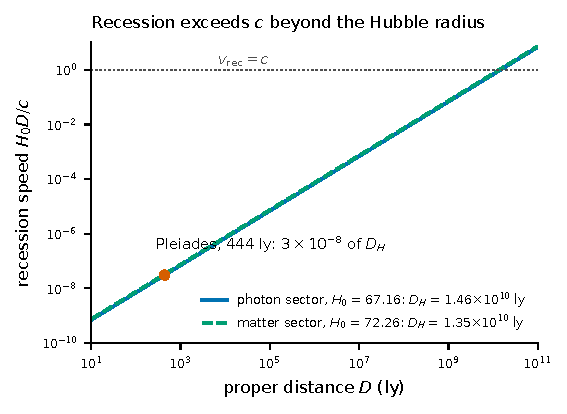
\includegraphics[width=0.62\textwidth]{figures/part7/fig_exploratory_recession.pdf}
\caption{Recession speed $H_0D/c$ against proper distance for the photon-sector ($H_0=67.16$) and matter-sector ($H_0=72.26$) expansion rates: it
reaches $c$ at the Hubble radius, $1.46$ and $1.35\times10^{10}$\,ly. The Pleiades (136\,pc~\cite{Melis2014}, 444\,ly) lie at $3\times10^{-8}$ of
it. Kinematics only; the energy conditions that stand in the way of a space-carrying drive are stated in Section~\ref{sec:ge_bubble}.
\calc}\label{fig:recession}
\end{figure}

\subsection{Proper time aboard a locally inertial bubble}\label{sec:ge_bubble}
Consider a craft enclosed in a region of locally flat spacetime that is itself displaced relative to distant stars by reshaping the surrounding geometry
(the mechanism is Zone~II; the kinematics here are not). The standard example is Alcubierre's metric~\cite{Alcubierre1994},
\begin{equation}
\mathrm ds^2=-c^2\mathrm dt^2+\left[\mathrm dx-v_s\,f(r_s)\,\mathrm dt\right]^2+\mathrm dy^2+\mathrm dz^2,\qquad
r_s=\sqrt{(x-x_s(t))^2+y^2+z^2},
\label{eq:ge_alc}
\end{equation}
with $v_s=\mathrm dx_s/\mathrm dt$ and a shape function $f$ equal to 1 inside the bubble and 0 far outside. Along the centre worldline,
$\mathrm dx=v_s\,\mathrm dt$ and $f=1$, so $\mathrm ds^2=-c^2\mathrm dt^2$. Inside a locally flat region the craft is inertial, so the proper time
elapsed aboard equals the coordinate time of the bubble's worldline,
\begin{equation}
\mathrm d\tau_{\rm ship}=\mathrm dt_{\rm bubble},
\label{eq:ge_tau}
\end{equation}
\derived{} and because the craft never acquires large local velocity through space, it accumulates none of the special-relativistic dilation factor
$\sqrt{1-v^2/c^2}$ that afflicts a near-$c$ through-space voyage. A clock at weak-field potential $\Phi$ runs at $\mathrm d\tau=(1+\Phi/c^2)\,\mathrm dt$.
Consequently the elapsed time on the craft and the elapsed time at the (comoving) origin differ only by the gravitational-potential term associated
with the engineered region,
\begin{equation}
\frac{\Delta\tau_{\rm Earth}-\Delta\tau_{\rm ship}}{\Delta\tau}\sim\frac{\Delta\Phi_{\rm IAM}}{c^2}\ll1
\label{eq:ge_dtau}
\end{equation}
for any potential small compared with $c^2$. \derived

\emph{Consequence (rigorous, conditional on a flat bubble existing).} A round trip that takes proper time $\Delta\tau_{\rm ship}$ aboard elapses
approximately the same $\Delta\tau_{\rm Earth}$ at the origin, in sharp contrast to relativistic through-space travel, where the twin asymmetry makes
$\Delta\tau_{\rm Earth}\gg\Delta\tau_{\rm ship}$ (Figure~\ref{fig:twin_exploratory}). This is the Alcubierre-class result: a space-carrying
displacement does not incur the twin-paradox penalty because the travellers remain locally inertial. It follows from the metric structure of a locally
flat displaced region. \derived{} (conditional)

The existence of such a region is where new physics is needed, and three published results stand against it. First, the energy density measured by
observers at rest in the slicing of Eq.~\eqref{eq:ge_alc} (lapse 1, shift $-v_sf$, flat spatial metric) follows from the Hamiltonian constraint
$16\pi G\rho/c^4=K^2-K_{ij}K^{ij}$; with $K_{ij}=\tfrac12(\partial_i\beta_j+\partial_j\beta_i)$ it is, in units $G=c=1$,
\begin{equation}
\rho=-\frac1{8\pi}\,\frac{v_s^2\,(y^2+z^2)}{4r_s^2}\left(\frac{\mathrm df}{\mathrm dr_s}\right)^2\le0 ,
\label{eq:ge_rho}
\end{equation}
negative wherever the wall has a slope off the axis, so the weak energy condition fails~\cite{Alcubierre1994}. \derived{} Second, quantum inequalities
confine negative energy to walls of near-Planck thickness and push the total requirement to enormous magnitudes~\cite{PfenningFord1997}. Third, for a
superluminal bubble the front wall is outside the causal reach of anyone inside it, so it can neither be made on demand nor controlled from
aboard~\cite{EverettRoman1997}. \derived{} (published results) These are the obstacles, and addressing them is the open problem for IAM as formulated.

\begin{figure}[htbp]\centering
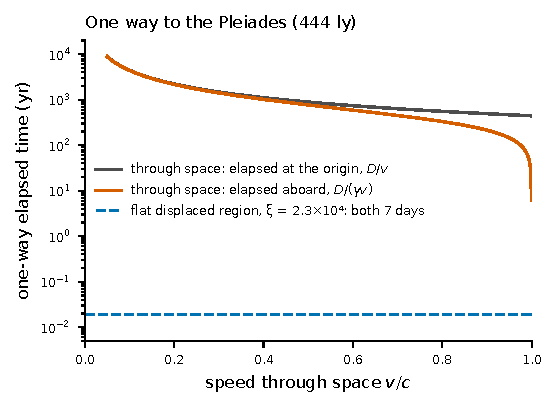
\includegraphics[width=0.62\textwidth]{figures/part7/fig_exploratory_twin.pdf}
\caption{One-way elapsed time to the Pleiades (444\,ly). Through space at constant $v$: $D/v$ at the origin and $D/(\gamma v)$ aboard (at $0.99c$,
448 and 63 years). In a flat displaced region carried at an effective rate $\xi c$ with $\xi=2.3\times10^4$, both clocks read 7 days to order
$\Delta\Phi/c^2$, Eq.~\eqref{eq:ge_dtau}; that region needs the negative energy density of Eq.~\eqref{eq:ge_rho}. \calc}\label{fig:twin_exploratory}
\end{figure}

\subsection{The transit figure for the Pleiades}
The Pleiades lie at $D\approx136$\,pc~\cite{Melis2014} $\approx444$ light-years. For a space-carrying displacement at effective rate $v_{\rm eff}=\xi c$
(with $\xi$ the ratio of induced proper-separation rate to $c$; $\xi>1$ is permitted because no local velocity exceeds $c$), the one-way coordinate time
is
\begin{equation}
t_{\rm one\text-way}=\frac{D}{v_{\rm eff}}=\frac{444\ \text{ly}}{\xi c}=\frac{444}{\xi}\ \text{years}.
\label{eq:ge_tone}
\end{equation}
By Section~\ref{sec:ge_bubble} the proper time aboard is approximately equal. A two-week round trip ($\Delta\tau_{\rm ship}\approx14$\,days, so
$t_{\rm one\text-way}\approx7\,\text{days}\approx0.0192$\,yr) requires
\begin{equation}
\xi=\frac{444\ \text{yr}}{0.0192\ \text{yr}}\approx2.3\times10^4 .
\label{eq:ge_xi}
\end{equation}
\calc{} That is, the surrounding geometry must be reshaped so that proper separation changes at $\sim2\times10^4$ $c$-equivalent. This number is not
forbidden by relativity (it is a rate of proper-separation change, not a local velocity), and 444 light-years is a negligible fraction,
$3\times10^{-8}$, of the Hubble radius of Eq.~\eqref{eq:ge_DH}. The distance to the Pleiades is not the obstacle; the negative energy density of
Eq.~\eqref{eq:ge_rho} is. What remains is the question of whether such a geometry can be engineered, which is Zone~II.

\begin{figure}[htbp]\centering
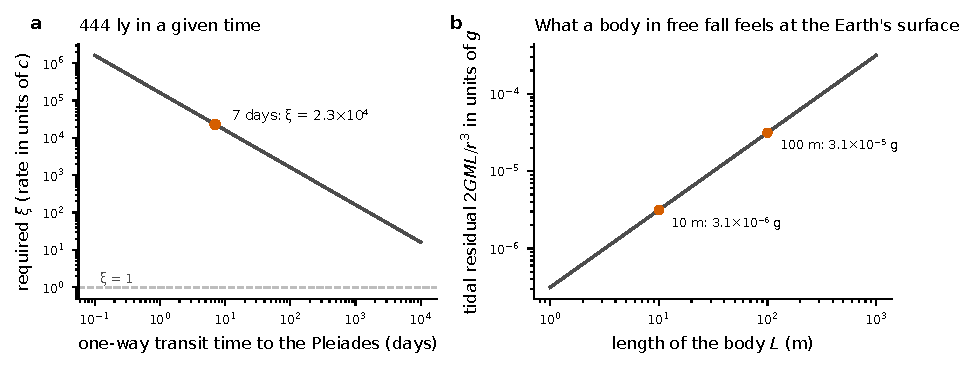
\includegraphics[width=\textwidth]{figures/part7/fig_exploratory_transit.pdf}
\caption{(a) The effective rate of proper-separation change, in units of $c$, that a one-way transit to the Pleiades (136\,pc~\cite{Melis2014},
444\,ly) requires, against transit time: $\xi=2.3\times10^4$ for seven days. Kinematics only. \calc\ (b) The tidal residual $2GML/r^3$ across a body of
length $L$ in free fall at the Earth's surface, in units of $g$: $3.1\times10^{-6}$ for 10\,m and $3.1\times10^{-5}$ for 100\,m; the uniform part of
the gradient is not felt. \derived}\label{fig:transit}
\end{figure}

\section{Transition to Zone II: conjecture begins here}\label{sec:ge_transition}
Everything above follows from established physics plus IAM's existing structure. What follows is conjecture. The remainder of this chapter concerns the
engineering coupling (how an external apparatus might write to the source of $\Phi_{\rm IAM}$ rather than merely read it) and the material that would
be required. Writing this coupling into IAM as currently formulated is the open derivation. It is conjectured to require a material (a long-lived island-of-stability superheavy held in macroscopic quantum coherence) whose existence is not established. This section therefore cannot be
derived. It states only the form that the missing physics would have to take, clearly labelled as conjecture, so that the structure of the open
problem is recorded. Each numbered item below is a premise or a conditional, never a result.

\section{Zone II: the conjectural engineering coupling}\label{sec:ge_zone2}

\subsection{The missing object: a coupling to the record-writing rate}
\textbf{Conjecture C1.} There exists a coupling by which a controlled physical input $J(\mathbf x,t)$ sources a local perturbation of the potential:
\begin{equation}
\Phi_{\rm IAM}(\mathbf x,t)=\Phi_0(\mathbf x)+\int G(\mathbf x-\mathbf x',t-t')\,J(\mathbf x',t')\,\mathrm d^3x'\,\mathrm dt'
\quad\text{(conjectured form; derivation open)},
\label{eq:ge_kernel}
\end{equation}
with $G$ a response kernel. \conjecture{} The kernel $G$ is unknown. IAM specifies that $\Phi_{\rm IAM}$ is sourced by the rate of irreversible record
writing; C1 conjectures that this rate can be driven rather than only observed. Deriving $G$ from the partition structure is the central open problem. \openprob

\subsection{The material premise}
\textbf{Premise P1 (knife-edge).} Driving the record-writing rate requires a substrate whose mass-energy is metastable with respect to the boundary
between coherent superposition and classical record, poised, so a small input tips a large mass-energy across in a controlled way. Ordinary matter is
fully decohered and does not respond. The island of stability (superheavy nuclei near the predicted shell closures, $Z\sim114$--126) is the conjectured
location of such metastable matter. \conjecture

\textbf{Premise P2 (coherence).} To hold an induced imbalance against the restoring tendency of the partition (the equilibrium that fixes the $1/2$
split), and to suppress the substrate's ordinary gravity-sourcing, the material must maintain macroscopic quantum coherence, i.e.\ be superconducting
in the operational state. \conjecture

\textbf{Tension.} P1 and P2 are in conflict in ordinary materials science: nuclear metastability and macroscopic electronic coherence are not known to
coexist. The conjecture is that the shell-closure structure granting the island its longevity may also support the ordered coherent state, i.e.\ that
the same magic numbers enable both. Whether this holds is open. \conjecture{} The superheavy nuclei made so far live from milliseconds to
seconds and are made a few atoms at a time~\cite{Oganessian2015}; no bulk sample exists to test. \observed{} Because this material is not known to exist, quantitative derivation past this point waits on its establishment, consistent with the principle that one cannot derive physics that requires an unestablished substrate.

\subsection{Predicted signature of the material, if it exists}
\textbf{Conditional prediction.} If P2 holds, a portion of the material's mass-energy is held in a coherent state, not yet written as a classical
record, and does not source gravity in proportion to its rest mass. Such a sample would exhibit an anomalous gravitational/inertial signature: it would
weigh slightly less than its measured mass-energy predicts. This is the one element of Zone~II that is empirically checkable should such a material
ever be produced: weigh it; if it is gravitationally anomalous, P2 is supported; if not, the conjecture fails. \prediction{} (conditional on the
material existing)

The test has a known baseline. A weight below the mass-energy is a difference between gravitational and inertial mass, a violation of the equivalence
principle. For ordinary materials the MICROSCOPE mission found the E\"otv\"os parameter of a titanium--platinum pair to be
$\eta({\rm Ti,Pt})=[-1.5\pm2.3\,({\rm stat})\pm1.5\,({\rm syst})]\times10^{-15}$~\cite{Touboul2022}, consistent with zero at $2.7\times10^{-15}$, and
lunar laser ranging confirms that gravitational binding energy itself gravitates as mass~\cite{Williams2004}. \observed{} For superconductors, the one
reported weight anomaly~\cite{Podkletnov1992} was not reproduced: two replication attempts found no change in the weight of a test
mass~\cite{Woods2001,Hathaway2003}, although neither reproduced the original apparatus, so that claim is neither confirmed nor excluded. \observed{} A
material with the proposed property would therefore have to differ from all tested matter, and a weighing at $10^{-15}$ or better would be the test.
\prediction{} (conditional)

\subsection{The steering geometry (conditional architecture)}\label{sec:ge_steer}
Conditional on C1 and a responsive material, the focal placement geometry follows from elementary field superposition. Sources at positions
$\mathbf r_i$, each driven with amplitude $A_i$ and phase $\phi_i$, produce a combined perturbation whose focal node $\mathbf x_f$ is steerable by
adjusting the relative $\{A_i,\phi_i\}$:
\begin{equation}
\Phi_{\rm drive}(\mathbf x)=\sum_i A_i\,G(\mathbf x-\mathbf r_i)\,e^{i\phi_i}\qquad\text{(conditional on the unknown }G).
\label{eq:ge_drive}
\end{equation}
Three facts about this sum need no knowledge of $G$ beyond its symmetry. \derived{} (geometry of superposition, conditional on $G$)
\begin{enumerate}
\item A focal node needs a time-dependent kernel. A static kernel that obeys Laplace's equation, such as $1/r$ ($\nabla^2(1/r)=0$ for $r>0$), has
no local maximum or minimum away from its sources (maximum principle), so a static superposition has no isolated focus. The phases $\phi_i$
in Eq.~\eqref{eq:ge_drive} therefore refer to an oscillating drive, and the focus is a maximum of the cycle-averaged $\langle|\Phi_{\rm drive}|^2\rangle$.
\item Two sources give only axial placement, and the monopole of one gives none.
\item For an isotropic kernel, $G=G(|\mathbf x-\mathbf r_i|)$, the field of any set of sources is symmetric under reflection in a plane that contains
them all. Three non-collinear sources therefore steer a single focal point only within their own plane; off that plane every focus has an equal mirror
twin (Figure~\ref{fig:steering}a). Placement of a single focal point throughout a 3D region needs at least four non-coplanar sources
(Figure~\ref{fig:steering}b), or a kernel that is not isotropic, such as directional emitters.
\end{enumerate}
With a few point sources the cycle-averaged field also has other maxima of comparable height (Figure~\ref{fig:steering}b), so a sharp, isolated node
needs either many sources or a kernel structure that is not yet known. \derived{} (illustrative kernel) The coherence premise P2 is what permits a
stable phase relation among the sources, hence a sharp (rather than noise-averaged) focal node. This is why the three elements (material, sources,
coherence) are jointly necessary and individually insufficient: the material supplies tippable mass-energy, the sources supply steerable aim, and
coherence couples the aim to the reservoir as a single phase-locked unit. \conjecture

\begin{figure}[htbp]\centering
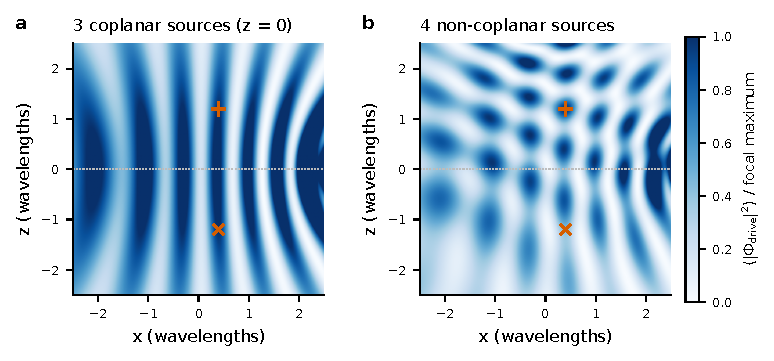
\includegraphics[width=\textwidth]{figures/part7/fig_exploratory_steering.pdf}
\caption{Cycle-averaged $|\Phi_{\rm drive}|^2$ of Eq.~\eqref{eq:ge_drive} in the $x$--$z$ plane, normalised to its value at the target ($+$), with
phases and amplitudes set to focus on the target, for an illustrative isotropic wave kernel $G=e^{ikr}/r$ (the true kernel is unknown). (a) Three
sources in the plane $z=0$: the field is mirror-symmetric about that plane, so the mirror point ($\times$) is an equal focus (ratio 1.00). (b) A fourth
source above the plane breaks the symmetry (mirror ratio 0.44), although other maxima of comparable height remain. \derived{} (symmetry; kernel
assumed for illustration)}\label{fig:steering}
\end{figure}

\subsection{What would close the gap}
The single derivation that would move the interstellar result from Zone~II to Zone~I is the response kernel $G$ of Eq.~\eqref{eq:ge_kernel}, derived
from the IAM partition structure, together with a demonstration that a material satisfying P1 and P2 can exist. A space-carrying displacement would also
need a source of the negative energy density of Eq.~\eqref{eq:ge_rho}, which neither general relativity with known matter nor IAM as formulated
supplies. \openprob{} Absent these, the kinematic results of Zone~I stand on their own. They state, rigorously, that if the geometry can be shaped, the
ride is weightless, the twin penalty is avoided, and 444 light-years is not the obstacle, while the engineering remains conjectural. The status of the whole is therefore: the destination is permitted by the kinematics; deriving the vehicle is the next step. \interp

\section{Summary}\label{sec:ge_summary}
\paragraph{Zone I (established).} Given IAM's identification of gravity as the gradient of an effective potential: a gradient-following craft feels no
acceleration during arbitrary maneuvers beyond the tidal term (equivalence principle); hover and abrupt departure follow as gradient operations; a
uniform gradient sets no orientation, so attitude is not a signature; the cosmological expansion already carries proper separations faster than $c$
without local violation; a locally flat displaced region avoids the twin-paradox penalty but needs negative energy density in its wall; and the
444 light-years to the Pleiades is a negligible fraction of the Hubble radius, requiring an effective rate $\xi\sim2\times10^4$ that relativity does not
forbid. These are consequences of existing physics plus IAM's existing structure.

\paragraph{Zone II (conjecture).} The engineering coupling that would let an apparatus drive (not merely observe) the source of the potential is not
derived and is not present in IAM as formulated; it is conjectured to require a metastable, macroscopically coherent superheavy material whose existence
is unestablished, with the one checkable prediction that such a material would weigh less than its mass-energy implies, against an
equivalence-principle baseline of $10^{-15}$ for all tested matter.

The boundary between these two zones is the content of this chapter. The kinematics say the stars are not as far as they look. General
relativity says the geometry that would carry a craft there needs negative energy, which no known matter supplies. Showing how to go is the engineering work that remains. These statements are true at once, and keeping them separate is the point. Zone~I is derivable from established physics and IAM structure;
Zone~II is explicitly conjectural. \interp

\begin{table}[htbp]\centering\small
\caption{Status of every result in this chapter.}\label{tab:ge_status}
\begin{tabularx}{\linewidth}{@{}>{\raggedright\arraybackslash}X>{\raggedright\arraybackslash}p{0.34\linewidth}@{}}\toprule
claim & status \\\midrule
Landauer cost per bit at $T_H$, Eq.~\eqref{eq:ge_landauer}; today's values & \calc \\\cmidrule[0.2pt]{1-2}
$E(1)=1$, $E\to e$, rate peak at $a=1$, Eq.~\eqref{eq:ge_Ea} & \derived \\\cmidrule[0.2pt]{1-2}
$\beta_m=\Omega_m/2$ & \derived{} (Chapter~\ref{ch:virial}) \\\cmidrule[0.2pt]{1-2}
two halves as gravitational potential and dark-energy term & \interp \\\cmidrule[0.2pt]{1-2}
$\mathbf g=-\nabla\Phi$, weak field, Eq.~\eqref{eq:ge_g} & \derived \\\cmidrule[0.2pt]{1-2}
no felt acceleration in free fall in a uniform gradient, Eq.~\eqref{eq:ge_felt} & \derived{} (equivalence principle) \\\cmidrule[0.2pt]{1-2}
tidal residual $2GML/r^3$; $3.1\times10^{-6}\,g$ (10\,m), $3.1\times10^{-5}\,g$ (100\,m) & \derived, \calc \\\cmidrule[0.2pt]{1-2}
hover $\nabla\Phi_{\rm IAM}=\mathbf g_{\rm amb}$; departure as a gradient setting & \derived{} (conditional on a shaped gradient) \\\cmidrule[0.2pt]{1-2}
hang angle of a suspended body, Eq.~\eqref{eq:ge_plumb} & \derived \\\cmidrule[0.2pt]{1-2}
no orientation set by a uniform gradient; gravity-gradient torque, Eq.~\eqref{eq:ge_ggtorque} & \derived \\\cmidrule[0.2pt]{1-2}
recession faster than $c$ beyond $D_H$; $D_H=1.46$, $1.35\times10^{10}$\,ly & \derived, \calc \\\cmidrule[0.2pt]{1-2}
expansion as the global expression of the kinetic half & \interp \\\cmidrule[0.2pt]{1-2}
a rate bound for a local region from $E\to e$ & \openprob{} (derivation open) \\\cmidrule[0.2pt]{1-2}
$\mathrm d\tau_{\rm ship}=\mathrm dt_{\rm bubble}$ inside a flat displaced region; no twin penalty & \derived{} (conditional on the region) \\\cmidrule[0.2pt]{1-2}
negative energy density in the wall, Eq.~\eqref{eq:ge_rho} & \derived{} (published) \\\cmidrule[0.2pt]{1-2}
quantum-inequality and causality obstacles & \derived{} (published) \\\cmidrule[0.2pt]{1-2}
Pleiades in seven days needs $\xi\approx2.3\times10^4$ & \calc \\\cmidrule[0.2pt]{1-2}
coupling C1 and kernel $G$, Eq.~\eqref{eq:ge_kernel} & \conjecture; derivation \openprob \\\cmidrule[0.2pt]{1-2}
premises P1, P2 and their reconciliation & \conjecture \\\cmidrule[0.2pt]{1-2}
superheavy nuclei: ms--s lifetimes, a few atoms at a time & \observed \\\cmidrule[0.2pt]{1-2}
weight anomaly of the coherent material & \prediction{} (conditional); ordinary matter $|\eta|\lesssim3\times10^{-15}$ \observed \\\cmidrule[0.2pt]{1-2}
steering: a static Laplace kernel has no focus; isotropic three-source mirror twin; four non-coplanar sources & \derived{} (conditional on $G$) \\\cmidrule[0.2pt]{1-2}
material, sources and coherence jointly necessary & \conjecture \\\bottomrule
\end{tabularx}
\end{table}

\section{Propulsion and the conservation laws}\label{sec:propulsion}

The propulsion material itself (gravity as the gradient of an effective potential, the weightless ride, the hover and
the abrupt departure, the expansion kinematics, the locally flat displaced region, the Pleiades transit figure, and the conjectured coupling,
material and steering sources) is set out above. This section adds the three checks that
any propulsion scheme has to pass before its kinematics mean anything: conservation of momentum, the universality of free fall, and the energy
conditions. The two zones keep their meaning. What follows from established physics and the law is marked \derived{} or \calc; what extends the
engineering past it is marked \conjecture. Nothing in this section is used anywhere else in the book.

\subsection{Zone I: momentum of a closed craft}\label{sec:pr_momentum}

\subsubsection{A craft cannot be pulled by its own field}
In this chapter the hover and the abrupt departure are both the same operation, shaping the gradient of $\Phi_{\rm IAM}$
(Eq.~\eqref{eq:ge_hover}), and the steering sources of Eq.~\eqref{eq:ge_drive} are part of one phase-locked unit with the material. Suppose the
sources ride with the craft. Write the field of a source distribution $\rho_B$ through a static kernel $G$ as
$\Phi_B(\mathbf x)=\int G(\mathbf x-\mathbf x')\rho_B(\mathbf x')\,\mathrm d^3x'$. The force of $B$'s field on a body $A$ and of $A$'s field on $B$ add to
\begin{equation}
\mathbf F_A+\mathbf F_B=-\iint\rho_A(\mathbf x)\,\rho_B(\mathbf x')\left[\nabla G(\mathbf x-\mathbf x')+\nabla G(\mathbf x'-\mathbf x)\right]\mathrm d^3x\,\mathrm d^3x' ,
\label{eq:pr_noforce}
\end{equation}
which vanishes for every pair whenever the kernel is even, $G(\mathbf u)=G(-\mathbf u)$, because its gradient is then odd. Newton's $1/r$, a Yukawa
kernel and any isotropic kernel are even. Summed over all parts of a craft, its own static field exerts no net force on it, however the field is
shaped. \derived{} A static kernel with an odd part would break the third law between the craft and its sources; in any translation-invariant field
theory momentum is conserved (Noether), so such a kernel would have to store the difference as field momentum. \derived

The hover and the departure therefore need one of three things that the gradient picture of this chapter does not supply: an
external body to push against, momentum carried away by the field, or matter of negative mass. Each has a price that can be computed. \derived

\subsubsection{Pushing on an external body}
If the engineered field acts between the craft and the Earth, the Earth takes the opposite momentum, exactly as it does under a walking person. A
hover is then a static balance between the craft and the planet below it: the field has to push the two apart with a force equal to the craft's
weight, and the planet is pushed down by the same amount. \derived{} A field that does this is the conjectured
coupling C1 of Section~\ref{sec:ge_zone2}, now required to act between two bodies, not only on one. \conjecture

\subsubsection{Throwing field momentum}
If the field carries momentum away, the craft recoils against it. For any field whose momentum density is bounded by its energy density over $c$
(electromagnetic and gravitational radiation, and any field that satisfies the dominant energy condition), the thrust per unit radiated power is at
most $1/c$:
\begin{equation}
F\le\frac{P}{c},\qquad P\ge m\,a\,c .
\label{eq:pr_thrust}
\end{equation}
\derived{} That is $3.34\times10^{-9}$\,N per watt. Holding one tonne at $1\,g$ takes $2.94\times10^{12}$\,W, and an abrupt departure at $100\,g$
takes $2.94\times10^{14}$\,W, for as long as it lasts. \calc{} A drive that works this way is a photon rocket whatever field it radiates, and the
weightless ride is paid for at the full rate of Eq.~\eqref{eq:pr_thrust}. \derived

\subsubsection{Negative mass}
The third way conserves momentum with no external reaction. A body of mass $+m$ and a body of mass $-m$ (inertial, passive and active masses all of the
same sign within each body) both accelerate in the same direction, from the negative toward the positive, each at $Gm/r^2$. Their total momentum
$mv+(-m)v$ and their total kinetic energy $\tfrac12mv^2+\tfrac12(-m)v^2$ stay zero as they speed up~\cite{Bondi1957}. \derived{} (published) This is the
self-propelled pair of Bondi's analysis of negative mass in general relativity. Its negative member has negative energy density, so it violates the
weak energy condition. \derived{} No known matter has negative mass. \observed

\subsection{Zone I: the universality of free fall}\label{sec:pr_universal}

\subsubsection{The weightless ride needs a universal field}
The weightless ride of Section~\ref{sec:ge_freefall} holds because every part of the craft and every occupant obeys the same equation of motion,
Eq.~\eqref{eq:ge_eom}. That is the equivalence principle, and it holds for gravity: the MICROSCOPE mission finds titanium and platinum falling alike to
about $10^{-15}$~\cite{Touboul2022} (Section~\ref{sec:ge_zone2}). \observed{} An engineered field is a different field. If it accelerates the hull
and the occupants at rates that differ by a fraction $\eta$, the occupants feel the difference,
\begin{equation}
f_{\rm felt}=m\,\eta\,a ,\qquad |\eta|\le\frac{\varepsilon\,g}{a}\ \text{to keep the felt load below }\varepsilon\,g .
\label{eq:pr_eta}
\end{equation}
\derived{} A departure at $100\,g$ felt below $0.01\,g$ needs $|\eta|\le10^{-4}$; a departure at $1000\,g$ felt below $0.1\,g$ needs the same. \calc{}
The premises of Section~\ref{sec:ge_zone2} make the drive material couple to gravity differently from ordinary matter (premise P2), so the field it
writes is not universal by construction, and whether it acts alike on hull, occupants and material is open. \conjecture{} Only a field that couples to
all mass-energy alike, as gravity does, gives the ride of Section~\ref{sec:ge_freefall}. \derived

\subsubsection{The tides of a steep focus}
The tidal residual of Eq.~\eqref{eq:ge_tidal} was evaluated in this chapter for the Earth's field. An abrupt departure needs a steep
gradient, and a steep gradient made by a focus close to the craft has large tides. For any field the tide across a craft of length $L$ is of order $aL/\ell$, where
$\ell$ is the distance over which the field changes. For a focus that acts as a monopole of strength $M$ at distance $r$, the acceleration is
$a=GM/r^2$ and the difference across the craft is
\begin{equation}
\Delta a=\frac{2GML}{r^3}=\frac{2aL}{r} .
\label{eq:pr_focus}
\end{equation}
\derived{} At $a=100\,g$ across $L=10$\,m the occupants feel $20\,g$ with the focus at 100\,m and $2\,g$ at 1\,km. Keeping the tide below
$0.01\,g$ needs the focus at least 200\,km away, and a focus there that pulls at $100\,g$ has the strength of $5.9\times10^{23}$\,kg, about a tenth of
the Earth's mass. \calc{} The free-fall argument removes the uniform part of the load; it does not remove this part. \derived

\subsection{Zone I: the energy conditions}\label{sec:pr_energy}

\subsubsection{Every superluminal displacement needs negative energy}
Section~\ref{sec:ge_bubble} gives the negative energy density in the wall of Alcubierre's region, Eq.~\eqref{eq:ge_rho}. The requirement is not
special to that metric. Defining superluminal travel as a path that reaches a destination surface earlier than any neighbouring path, and assuming
the generic condition, Olum proved that any such travel requires a violation of the weak energy condition, that is, negative energy
density~\cite{Olum1998}. \derived{} (published) The rate $\xi=2.3\times10^4$ of the Pleiades transit, Eq.~\eqref{eq:ge_xi}, is superluminal in this
sense, so whatever geometry carries it has negative energy somewhere. \derived

\subsubsection{How much}
Integrating Eq.~\eqref{eq:ge_rho} over a constant-time slice, with $\int(y^2+z^2)/r^2\,\mathrm d\Omega=8\pi/3$, gives in units $G=c=1$
\begin{equation}
E=-\frac{v_s^2}{12}\int_0^\infty r^2\left(\frac{\mathrm df}{\mathrm dr}\right)^2\mathrm dr ,
\label{eq:pr_Etot}
\end{equation}
\derived{} and for a wall of thickness $\Delta$ at radius $R$, with $f$ falling linearly across the wall,
\begin{equation}
E=-\frac{v_s^2}{12}\left(\frac{R^2}{\Delta}+\frac{\Delta}{12}\right) ,
\label{eq:pr_Ewall}
\end{equation}
as Pfenning and Ford give it~\cite{PfenningFord1997}; the smooth $\tanh$ wall of Alcubierre's shape function gives $R^2\sigma/3$ for the integral, the
same form with $\sigma=3/\Delta$. \derived{} The quantum inequalities hold the wall to $\Delta\le10^2\,v_s\,L_{\rm P}$~\cite{PfenningFord1997}.
For a bubble of radius 100\,m at $v_s=c$ that is $|E|=6.9\times10^{62}$\,kg, which Pfenning and Ford put at $6.2\times10^{62}$\,kg, or
$3\times10^{20}$ galaxies of $2\times10^{42}$\,kg~\cite{PfenningFord1997}. \calc{} At the Pleiades rate $v_s=2.3\times10^4\,c$, taking their wall
bound at face value, $|E|=1.6\times10^{67}$\,kg. \calc{} A wall 1\,m thick, which the quantum inequalities forbid, would need $0.56$ solar masses at
$v_s=c$. \calc{} These magnitudes are the obstacle that this chapter names; IAM as formulated supplies no negative energy and no way
around Olum's theorem. \derived

\subsection{Zone II: what the weighing test would measure}\label{sec:pr_weigh}

\subsubsection{Active and passive mass}
The conditional prediction of Section~\ref{sec:ge_zone2} states two properties of the coherent material at once: it does not source gravity in
proportion to its rest mass, and it would weigh less than its mass-energy predicts. These are two different masses. The mass that sources gravity is
the active gravitational mass $m_a$; the mass that a field pulls on, which a balance weighs, is the passive gravitational mass $m_p$. For two bodies
held at fixed separation $r$ the forces do not cancel unless the ratio of the two masses is the same for both:
\begin{equation}
F_{\rm net}=\frac{G\,m_{p1}m_{p2}}{r^2}\left(\frac{m_{a2}}{m_{p2}}-\frac{m_{a1}}{m_{p1}}\right) .
\label{eq:pr_selfforce}
\end{equation}
\derived{} A material whose ratio differs from that of ordinary matter would make any rigid object built from both accelerate by itself, against the
conservation of momentum. Lunar laser ranging finds the ratio the same for aluminium and iron to $4\times10^{-12}$~\cite{BartlettVanBuren1986} and
now to $3.9\times10^{-14}$~\cite{Singh2023}. \observed{} The weighing of Section~\ref{sec:ge_zone2} tests $m_p$; a torsion-balance attraction tests
$m_a$. The conjecture as written changes both. \conjecture{} They have to change in the same ratio, or momentum is not conserved. \derived

\subsubsection{Hover by weight reduction}
If the drive material of mass $m_d$ weighs a fraction $\delta$ less, $(1-\delta)\,m_d$, and carries an ordinary payload $m_{\rm pay}$, the whole
craft weighs nothing when
\begin{equation}
(1-\delta)\,m_d+m_{\rm pay}=0,\qquad \delta=1+\frac{m_{\rm pay}}{m_d} .
\label{eq:pr_hover}
\end{equation}
\derived{} The fraction is larger than one for any payload: $\delta=2$ for a payload as heavy as the drive, which makes the passive mass of the drive
$-m_{\rm pay}$. A self-contained craft that hovers by weighing less needs drive material of negative passive mass, not material that weighs slightly
less. \derived{} A small anomaly, if one were ever found, would support premise P2 but would not by itself lift anything. \conjecture

\subsection{Summary}\label{sec:pr_summary}
\paragraph{Zone I (established).} A craft whose sources ride with it cannot be moved by its own static field (Eq.~\eqref{eq:pr_noforce}). A hover or
departure needs an external body to push on, radiated field momentum at $P\ge mac$ ($2.94\times10^{12}$\,W per tonne at $1\,g$), or negative mass.
The weightless ride holds only for a field that acts alike on all mass-energy, to $|\eta|\le\varepsilon g/a$, and a steep focus adds the tide
$2aL/r$, $20\,g$ across 10\,m at 100\,m from a $100\,g$ focus. Every superluminal displacement needs negative energy (Olum), $6.9\times10^{62}$\,kg
for a 100\,m bubble at $c$ and $1.6\times10^{67}$\,kg at the Pleiades rate. \derived, \calc

\paragraph{Zone II (conjecture).} The coherent material has to change its active and passive gravitational mass together, or momentum is not
conserved (lunar ranging holds aluminium and iron to $3.9\times10^{-14}$); and a self-contained craft that hovers by weighing less needs negative
passive mass, $\delta=1+m_{\rm pay}/m_d$. \conjecture

The kinematics of this chapter say where the stars are. The conservation laws say what any vehicle would have to pay to get there:
momentum to something, energy below zero, and a field that pulls on everything alike. \interp

\begin{table}[htbp]\centering\small
\caption{Status of every result in this section.}\label{tab:pr_status}
\begin{tabularx}{\linewidth}{@{}>{\raggedright\arraybackslash}X>{\raggedright\arraybackslash}p{0.34\linewidth}@{}}\toprule
claim & status \\\midrule
no net force of a craft's own static field, even kernel, Eq.~\eqref{eq:pr_noforce} & \derived \\\cmidrule[0.2pt]{1-2}
an odd static kernel breaks the third law; momentum stored in the field & \derived \\\cmidrule[0.2pt]{1-2}
hover against an external body needs coupling C1 between two bodies & \conjecture \\\cmidrule[0.2pt]{1-2}
thrust from field momentum $F\le P/c$; $2.94\times10^{12}$\,W per tonne at $1\,g$, $2.94\times10^{14}$\,W at $100\,g$ & \derived, \calc \\\cmidrule[0.2pt]{1-2}
negative-mass pair self-accelerates with momentum and energy conserved & \derived{} (published) \\\cmidrule[0.2pt]{1-2}
no known matter has negative mass & \observed \\\cmidrule[0.2pt]{1-2}
felt load $m\eta a$; $|\eta|\le10^{-4}$ for $100\,g$ felt below $0.01\,g$, Eq.~\eqref{eq:pr_eta} & \derived, \calc \\\cmidrule[0.2pt]{1-2}
universality of the engineered field & \conjecture \\\cmidrule[0.2pt]{1-2}
tide of a monopole focus $2aL/r$; $20\,g$, $2\,g$; 200\,km and $5.9\times10^{23}$\,kg for $0.01\,g$, Eq.~\eqref{eq:pr_focus} & \derived, \calc \\\cmidrule[0.2pt]{1-2}
pair self-force from unequal $m_a/m_p$, Eq.~\eqref{eq:pr_selfforce} & \derived \\\cmidrule[0.2pt]{1-2}
$m_a/m_p$ equal for Al and Fe to $4\times10^{-12}$, $3.9\times10^{-14}$ & \observed \\\cmidrule[0.2pt]{1-2}
active and passive mass of the material change together & \conjecture \\\cmidrule[0.2pt]{1-2}
hover by weight reduction needs $\delta=1+m_{\rm pay}/m_d>1$, Eq.~\eqref{eq:pr_hover} & \derived \\\cmidrule[0.2pt]{1-2}
superluminal travel requires negative energy density & \derived{} (published) \\\cmidrule[0.2pt]{1-2}
total negative energy $-(v_s^2/12)(R^2/\Delta+\Delta/12)$, Eqs.~\eqref{eq:pr_Etot}, \eqref{eq:pr_Ewall} & \derived \\\cmidrule[0.2pt]{1-2}
$6.9\times10^{62}$\,kg (100\,m, $c$); $1.6\times10^{67}$\,kg ($2.3\times10^4c$); $0.56\,M_\odot$ (1\,m wall) & \calc \\\bottomrule
\end{tabularx}
\end{table}

Zone~I is established physics, and Zone~II is stated as conjecture with every obstacle named. A physicist who wants to work on the engineering coupling now knows exactly what a derivation would have to deliver.
